\documentclass{beamer}
\usepackage{../../ikany}

\usepackage[small]{eulervm}
\usefonttheme{professionalfonts}
\usefonttheme[onlymath]{serif}

\title{Diachrony of Spectra}
\author{Ikhan Choi}

\begin{document}
\maketitle

\begin{frame}
\frametitle{Introduction}
  \pause
  \begin{defn}
    Let $R$ be a commutative ring.
    The \emph{spectrum} of $R$ is the set of prime ideals of $R$.
  \end{defn}
  \pause
  \begin{ex}
  	\[\Spec(\Z)=\{\,2\Z,3\Z,5\Z,7\Z,11\Z,\cdots\,\}.\]
  \end{ex}
  \pause
  \begin{qn}
    Why is it defined like this?
  \end{qn}
\end{frame}


\section{Hydrogen atom}

\begin{frame}
\frametitle{Contents}
  \tableofcontents[currentsection]
\end{frame}

\begin{frame}
\frametitle{Hydrogen spectral series}
  \begin{figure}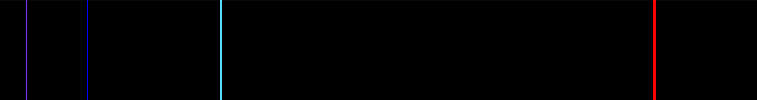
\includegraphics[scale=.4]{emission.png}\end{figure}
  \pause 410.2nm \hspace{2em} 468.1nm \hspace{12em} 656.3 nm\\ \hspace{2em} 434.0nm\\
  \bigskip
  \pause
  \begin{qn}
    How can we explain and compute this phenomenon?
  \end{qn}
\end{frame}

\begin{frame}
\frametitle{Rydberg's formula : Bohr model}
  Bohr's postulates:\pause
  \begin{itemize}[<+->]
    \item The electrons are on certian stable orbits.
    \item The stationary orbits are computed by the old quantization assumption for angular momenta:
    \[mvr=n\hslash.\]
    \item An electron absorbs or emits light frequency $f$ when they jump from an orbit to another, satisfying
    \[\Delta E=hf.\]
  \end{itemize}
  \uncover<5->{The constant $h$ is called the Planck constant and $\hslash:=\frac h{2\pi}$.}
\end{frame}

\begin{frame}
\frametitle{Rydberg's formula : Bohr model}
  From the three relations
  \[mvr=n\hslash,\quad\frac{mv^2}r=-k\frac{(+e)(-e)}{r^2},\quad E=K+V=\frac12mv^2-k\frac{e^2}r,\]
  \pause we deduce
  \[E=-\frac{k^2e^4m}{2\hslash^2}\frac1{n^2}\approx-13.6\frac1{n^2}\ (eV).\]
  \pause
  \begin{prop}[Rydberg formula]
    The wavelengths $\lambda$ of absorbed or emitted photons from a hydrogen atom is estimated by the following formula:
    \[\frac1\lambda=R\left(\frac1{n_1^2}-\frac1{n_2^2}\right),\c{for}n_1,n_2\in\N,\]
    where $R:=\frac{k^2e^4m}{4\pi\hslash^3c}$ is the \emph{Rydberg constant}.
  \end{prop}
\end{frame}

\begin{frame}
\frametitle{Rydberg's formula : Schr\"odinger equation}
  More mathematically!\\
  \pause In quantum mechanics, an electron around a hydrogen atom is described by the Schr\"odinger equation: for $(t,x)\in\R^{1+3}$
  \[i\hslash\pd{t}\Psi(t,x)=-\frac{\hslash^2}{2m}\del^2\Psi(t,x)+V(x)\Psi(t,x),\]
  \pause \hspace{5em} energy \hspace{2em} kinetic energy \hspace{1em} potential energy\\
  \bigskip
  \pause where $V$ is given by the Coulomb potential
  \[V(x)=-\frac2{|x|}.\]
  \pause By solving it, we obtain the probability distribution $|\Psi(t,x)|^2$ of the electron at time $t$.
  \pause Let's solve.
\end{frame}

\begin{frame}
\frametitle{Rydberg's formula : Schr\"odinger equation}
  Schr\"odinger equation:
  \[i\hslash\pd{\Psi(t,x)}{t}=-\frac{\hslash^2}{2m}\del^2\Psi(t,x)+V(x)\Psi(t,x).\]
  \pause ``Mathematization'':
  \[i\pd_t\Psi(t,x)=(-\Delta+V(x))\Psi(t,x).\]
  \pause
  Ansatz: if the solutions has the form $\Psi(t,x)=\phi(t)\psi(x)$, then\pause
  \[\frac{i\pd_t\phi(t)}{\phi(t)}=\frac{(-\Delta+V(x))\psi(x)}{\psi(x)}\pause=E.\]
  \pause The constant $E$ is interpreted as the energy of electrons.
  \pause We have two \emph{eigenvalue problems} with \emph{shared eigenvalue} $E$:\pause
  \begin{gather*}
    i\dd{t}\phi(t)=E\phi(t),\\
    (-\Delta+V(x))\psi(x)=E\psi(x).
  \end{gather*}
\end{frame}

\begin{frame}
\frametitle{Rydberg's formula : Schr\"odinger equation}
  Suppose we already have found the solutions $\phi_E(t)$, $\psi_E(x)$ of the eigenvalue problems for each complex number $E$.\pause
  \begin{itemize}[<+->]
    \item All functions of the form \[\Phi(t,x)=\sum_Ec_E\psi_E(t)\phi_E(x)\] are solutions of the original Schr\"odinger equation(in fact we can find all solutions in this way).
    \item For a given $E$, $\phi_E$ and $\psi_E$ are of course not unique. In fact they form a vector space which is called the eigenspace.
    \item Note that for some $E$ we probably cannot find the solution $\psi_E(x)$ that satisfies $\int|\psi_E(x)|^2\,dx=1$: the eigenspace is trivial.
    \item Since $\phi_E(t)\propto e^{-iEt}$ is easily solved, the main difficulty is $\psi_E$.
  \end{itemize}
  \begin{rmk}
    The first one is not mathematically correct statement because we should resolve some technical issues on convergence.
  \end{rmk}
\end{frame}

\begin{frame}
\frametitle{Rydberg's formula : Schr\"odinger equation}
  So, what we need to investigate seriously is:
  \pause\emph{what are the eigenvalues and eigenvectors of the operator}
  \[\cH:L^2(\R^3)\to L^2(\R^3)\]
  \emph{defined by}
  \[\cH\psi(x):=(-\Delta-|x|^{-1})\psi(x)?\]
  \emph{Also, how can we compute them?}
  \pause \[\textbf{The Beginning of Spectral Theory}\]
\end{frame}

\begin{frame}
\frametitle{Rydberg's formula : Schr\"odinger equation}
  With long long calculations and hard hard mathematics, experts found the following result:
  \begin{prop}
    The eigenvalues of $\cH=-\Delta-2|x|^{-1}$ are
    \[-1,-\frac14,-\frac19,-\frac1{16},\cdots\]
    \pause with multiplicity $1$, $1+3$, $1+3+5$, $1+3+5+7$, and so on.
  \end{prop}
  \pause Since the eigenvalues embody the possible energy values of an electron, we just gave the Rydberg formula a reasonable explanation.
  \pause This result explains not only the discretized energy spectrum but also the number of each orbitals!
\end{frame}

\section{Spectral theory of elliptic equations}
\begin{frame}
\frametitle{Contents}
  \tableofcontents[currentsection]
\end{frame}

\begin{frame}
\frametitle{Separation of variables}
\end{frame}
\begin{frame}
\frametitle{Spectral theorem of normal matrices}
\end{frame}
\begin{frame}
\frametitle{Spectral theorem of compact operators}
\end{frame}
\begin{frame}
\frametitle{Spectral theorem of elliptic operators}
\end{frame}


\section{Gelfand theory}
\begin{frame}
\frametitle{Banach algebras and $C^*$-algebras}
\end{frame}
\begin{frame}
\frametitle{Example 1 : Bounded operators}
\end{frame}
\begin{frame}
\frametitle{Example 2 : Continuous functions}
\end{frame}
\begin{frame}
\frametitle{Spectra, multiplicative homomorphisms, maximal ideals}
\end{frame}
\begin{frame}
\frametitle{Gelfand-Naimark theorem}
\end{frame}


\section{Algebraic geometry}
\begin{frame}
\frametitle{Algebraic variety}
\end{frame}
\begin{frame}
\frametitle{Coordinate ring}
\end{frame}
\begin{frame}
\frametitle{Maximal ideal is a point}
\end{frame}
\begin{frame}
\frametitle{Problem of unified codomains}
\end{frame}
\begin{frame}
\frametitle{Functoriality}
\end{frame}

\end{document}